\documentclass[../presentation.tex]{subfiles} % Parent file
\graphicspath{{\subfix{../images/}}} % Images path

\begin{document}

\section{Datasets}

\begin{frame}

    \frametitle{Brain Tumor MRI Dataset}

    \begin{cbox}
        \begin{itemize}
            \item Combination of three datasets
            \item 7023 images of human brain MRI images
            \item Four classes: glioma, meningioma, no-tumor and pituitary
        \end{itemize}
    \end{cbox}

    \vspace{0.2cm}

    \begin{center}
        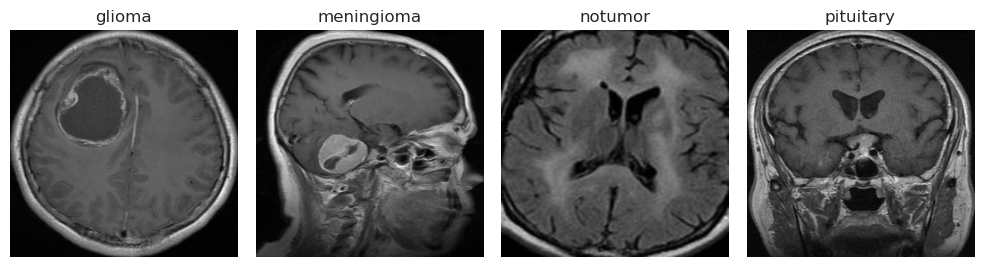
\includegraphics[width=1\textwidth]{classification_samples.png}
    \end{center}

\end{frame}

\begin{frame}
    
    \frametitle{Brain Tumor MRI Dataset}

    \begin{cbox}
        The dataset is separated into training and testing sets with a ratio of 80\% and 20\% respectively
    \end{cbox}

    \begin{center}
        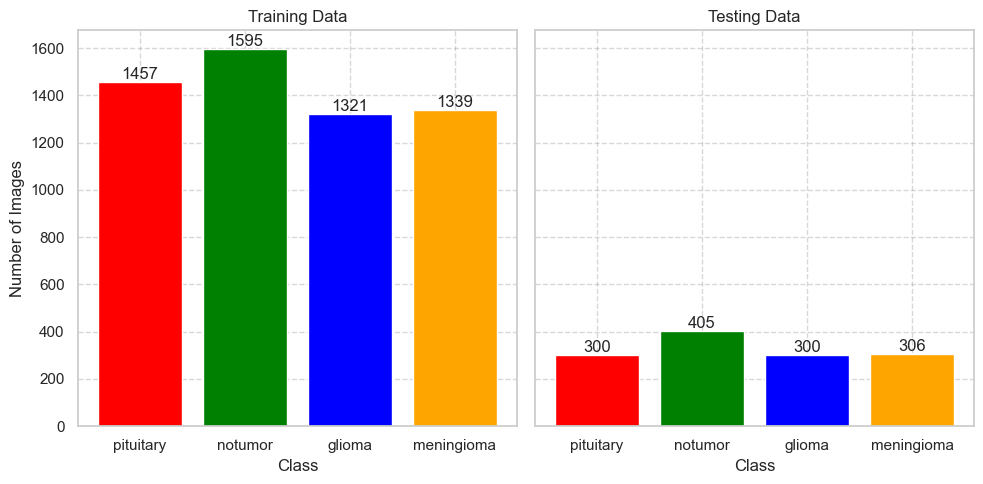
\includegraphics[width=1\textwidth]{classification_dataset_histo.png}
    \end{center}

\end{frame}

\end{document}
